\addcontentsline{toc}{chapter}{Занятие 4. Гауссовские процессы}
\chapter*{Занятие 4. Гауссовские процессы}

\addcontentsline{toc}{section}{Контрольные вопросы и задания}
\section*{Контрольные вопросы и задания}

\subsubsection*{Приведите определение гауссовского процесса.}

Процесс $ \left\{ X \left( t \right), \, t \in T \right\} $ --- гауссовский, если
$$ \sum \limits_{k = 1}^n \lambda_k X \left( t_k \right) $$
--- гауссовская случайная величина $ \forall \vec{ \lambda } \in \mathbb{R}^n$ и
$ \forall t_1, \dotsc, t_n \in T$.

Эквивалентно: $ \left( X \left( t_1 \right), \dotsc, X \left( t_n \right) \right)^T$ ---
гауссовский вектор.

\subsubsection*{Запишите плотность конечномерных распределений гауссовского процесса.}

$$p =
  \frac{1}{ \left( \sqrt{2 \pi} \right)^n} \cdot \frac{1}{ \sqrt{det \, A}} \cdot
  e^{-\frac{1}{2} \left[ A^{-1} \left( \vec{x} - \vec{a} \right), \vec{x} - \vec{a} \right] },$$
если $det \, A > 0$.
Квадратные скобки в степени экспоненты --- это скалярное произведение,
или квадратичная форма матрицы, обратной к ковариации.

\subsubsection*{Приведите определение и сформулируйте основные свойства ковариационной функции.}

$K \left( t, s \right) =
  cov \left[ X \left( t \right), X \left( s \right) \right] $.

Гауссовский процесс существует, из теомеры Колмогорова, с функциями $m$ и $K$ тогда и только тогда,
когда функция $K \left( s, t \right) = K \left( t, s \right) $ --- симметричная, и $K$ ---
неотрицательно определённая, то есть
$$ \sum \limits_{k, j = 1}^n c_k c_j K \left( t_k, t_j \right) \geq
  0.$$

Тут неравенство возможно для любых $c_1, \dotsc, c_n, t_1, \dotsc, t_n$.

\subsubsection*{4.2}

\textit{Задание.}
Выясните, существует ли случайный процесс с ковариационной функцией
\begin{enumerate}[label=\alph*)]
  \item $K \left( t, s \right) = \min \left( t, s \right) $;
  \item $K \left( t, s \right) =
    \left( 1 - \left| t - s \right| \right) \cdot
    \mathbbm{1} \left\{ \left| t - s \right| < 1 \right\}; \,
    t, s \in \mathbb{R}$.
\end{enumerate}

\textit{Решение.}
\begin{enumerate}[label=\alph*)]
  \item $K \left( t, s \right) = \min \left( t, s \right) $.

  Такой процесс есть.
  Какой?
  Винеровский;
  \item $K \left( t, s \right) =
    \left( 1 - \left| t - s \right| \right) \cdot
    \mathbbm{1} \left\{ \left| t - s \right| < 1 \right\}; \,
    t, s \in \mathbb{R}$.

  Если такой процесс есть, то мы его не встречали раньше.
  Симметричность очевидна.
  Вопрос: будет ли такая функция неотрицательно определена?

  Функция зависит только от разности.
  Сейчас $K \left( t, s \right) = \varphi \left( t - s \right) $, где
  $$ \varphi \left( t \right) =
    \begin{cases}
      1 - \left| t \right| , \qquad \left| t \right| \leq 1, \\
      0, \qquad \left| t \right| > 1.
    \end{cases}$$
  Так что
  $$ \sum \limits_{k, j = 1}^n c_k c_j K \left( t_k, t_j \right) =
    \sum \limits_{k, j = 1}^n c_k c_j \varphi \left( t_k - t_j \right) \geq
    0$$
  --- это условие неотрицательной определённости для характеристической функции.
  Будет ли эта функция $ \varphi $ характеристической?
  То есть вопрос в задаче равносилен следующему: будет ли
  $$ \varphi \left( t \right) =
    \begin{cases}
      1 - \left| t \right| , \qquad \left| t \right| \leq 1, \\
      0, \qquad \left| t \right| > 1.
    \end{cases}$$
  характеристической функцией?
  Эта функция изображена на рисунке \ref{fig:42}.

  \begin{figure}[h!]
    \centering
    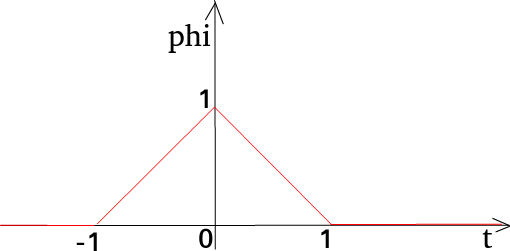
\includegraphics[width=.4\textwidth]{./pictures/4_2.png}
    \caption{График функции $ \varphi \left( t \right) $}
    \label{fig:42}
  \end{figure}


  Она непрерывная, симметричная, в нуле --- единица.
  Если бы это была характеристическая функция
  $$ \varphi \left( t \right) =
    \int \limits_{-\infty }^{+\infty } e^{itx} p \left( x \right) dx$$
  --- преобразование Фурье плотности $p \left( x \right) $.
  Плотность можно найти через обратное преобразование Фурье
  $$p \left( x \right) =
    \frac{1}{2 \pi } \int \limits_{-\infty}^{+\infty } e^{-itx} \varphi \left( t \right) dt =
    \frac{1}{2 \pi } \int \limits_{-1}^1 e^{-itx} \left( 1 - \left| t \right| \right) dt =$$
  Раскроем модуль
  $$= \frac{1}{2 \pi } \left(
    \int \limits_{-1}^1 e^{-itx} dt + \int \limits_{-1}^0 e^{-itx} tdt -
    \int \limits_0^1 e^{-itx} tdt \right) =$$
  Берём первый интеграл
  $$= \frac{1}{2 \pi } \left(
    \left. -\frac{e^{-itx}}{ix} \right|_{-1}^1 - \int \limits_0^1 e^{itx} tdt -
    \int \limits_0^1 e^{-itx} tdt \right) =$$
  Подставляем пределы интегрирования
  $$= \frac{1}{2 \pi } \left[
    -\frac{e^{-ix}}{ix} + \frac{e^{ix}}{ix} -
    \int \limits_0^1 \left( e^{-itx} + e^{itx} \right) tdt \right] =$$
  Из формулы Эйлера следует, что $e^{-itx} + e^{itx} = 2 \cos \left( tx \right) $.
  Тогда
  $$= \frac{1}{2 \pi }
    \left[ \frac{-e^{-ix} + e^{ix}}{ix} - 2 \int \limits_0^1 \cos \left( tx \right) tdt \right] =$$
  Интегрируем по частям, то есть
  $$u = t, \,
    du = dt, \,
    dv = \cos \left( tx \right) dt, \,
    c = \int \cos \left( tx \right) dt = \frac{1}{x} \cdot \sin \left( xt \right).$$
  Получаем
  $$= \frac{1}{2 \pi } \left[
      \frac{-e^{-ix} + e^{ix}}{ix} -
      2 \cdot \left. \frac{t}{x} \cdot \sin \left( xt \right) \right|_0^1 +
      2 \int \limits_0^1 \frac{1}{x} \cdot \sin \left( xt \right) dt \right] =$$
  Подставляем пределы интегрирования и берём интеграл от синуса
  $$= \frac{1}{2 \pi } \left[
    \frac{-e^{-ix} + e^{ix}}{ix} - \frac{2}{x} \cdot \sin x -
    \left. \frac{2}{x^2} \cdot \cos \left( xt \right) \right|_0^1 \right] =$$
  Снова подставляем пределы интегрирования
  $$= \frac{1}{2 \pi } \left(
    \frac{-e^{-ix} + e^{ix}}{ix} - \frac{2}{x} \cdot \sin x - \frac{2}{x^2} \cdot \cos x +
    \frac{2}{x^2} \right) =$$
  Из формулы Эйлера следует, что $e^{ix} - e^{-ix} = 2i \sin x$.
  Тогда
  $$= \frac{1}{2 \pi} \left[
    \frac{2 \sin x}{x} - \frac{2 \sin x}{x} + \frac{2}{x^2} \left( -\cos x + 1 \right) \right] =
  \frac{1}{ \pi x^2} \left( 1 - \cos x \right).$$

  Нашли обратное преобразование Фурье
  $$ \varphi \left( t \right) =
    \int \limits_{-\infty }^{+\infty } e^{itx} p \left( x \right) dx $$
  и $p \left( x \right) \geq 0$.

  Должно выполняться условие нормировки
  $$ \int \limits_{-\infty }^{+\infty } p \left( x \right) dx =
    \varphi \left( 0 \right) =
    1.$$
  Так что $p$ --- плотность, $ \varphi $ --- это её преобразование Фурье, так что $ \varphi $ ---
  характеристическая функция.
  \end{enumerate}

\subsubsection*{4.3}

\textit{Задание.}
Пусть $K \left( t, s \right), \, t, s \in T$ ---
ковариационная функция некоторого случайного процесса, $Q \left( t \right) $ ---
полином с положительными коэффициентами.
Докажите, что функция $K_1 \left( t, s \right) = Q \left( K \left( t, s \right) \right) $
тоже является ковариационной функцией некоторого случайного процесса.

\textit{Решение.}
$Q \left( t \right) = a_0 + a_1 t + a_2 t^2 + \dotsc + a_n t^n, \, a_0, a_1, \dotsc, a_n \geq 0$.
Доказать, что если в этот многочлен подставить ковариационную функцию,
то снова получится ковариационная функция.

Явно запишем, что такое
$$K_1 \left( t, s \right) =
  a_0 + a_1 K \left( t, s \right) + a_2 K \left( t, s \right)^2 + \dotsc +
  a_n K \left( t, s \right)^n.$$

Симметричность есть, так как $K \left( t, s \right) $ --- симметрична.

Задачу можно разбить на две подзадачи:
\begin{enumerate}
  \item если $R_0, R_1, R_2, \dotsc, R_n$ --- ковариационные функции, то и
  $$ \sum \limits_{j = 0}^n a_j R_j \left( t, s \right) $$
  --- ковариационная функция.
  Это утверждение проверить просто.

  Доказательство.
  Берём двойную сумму
  $$ \sum \limits_{k, i = 1}^n
    c_k c_i \left( \sum \limits_{j = 0}^n a_j R_j \left( t_k, t_i \right) \right) =$$
  Меняем суммы местами
  $$= \sum \limits_{j = 0}^n
    a_j \left( \sum \limits_{k, i = 1}^n R_j \left( t_k, t_i \right) c_k c_i \right) \geq 0,$$
  так как внутренняя сумма неотрицательна.
  Так что 1. проверили;
  \item чтобы 1. применить, достаточно проверить, что степень ковариационной функции ---
  это тоже ковариационная функция.
  Достаточно проверить, что если $R_1, R_2$ --- ковариационные функции,
  то и произведение $R_1 \left( t, s \right) R_2 \left( t, s \right) $ ---
  тоже ковариационная функция.

  Условие неотрицательности сейчас записывается так
  $$ \sum \limits_{k, j = 1}^n c_k c_j R_1 \left( t_k, t_j \right) R_2 \left( t_k, t_j \right) \geq
    0?,$$
  где
  $R_1 \left( t_k, t_j \right) = M \left[ X \left( t_k \right) X \left( t_j \right) \right], \,
    R_2 \left( t_k, t_j \right) = M \left[ Y \left( t_k \right) Y \left( t_j \right) \right] $.

  Раз $R_1$ --- ковариационая и $R_2$ --- ковариационная,
  то существуют независимые процессы $X \left( t \right) $ и $Y \left( t \right) $, такие, что
  $$R_1 \left( t, s \right) = M \left[ X \left( t \right) X \left( s \right) \right], \,
    R_2 \left( t, s \right) = M \left[ Y \left( t \right) Y \left( s \right) \right].$$
  Тогда если возьмём новый процесс
  $$Z \left( t \right) = X \left( t \right) Y \left( t \right),$$
  то
  $M \left[ Z \left( t \right) Z \left( s \right) \right] =
    M \left[ X \left( t \right) Y \left( t \right) X \left( s \right) Y \left( s \right) \right] $.
  Группируем первый множитель с третьим, второй --- с четвёртым, пользуемся независимостью
  $M \left[ X \left( t \right) Y \left( t \right) X \left( s \right) Y \left( s \right) \right] =
    M \left[ X \left( t \right) X \left( s \right) \right] \cdot
    M \left[ Y \left( t \right) Y \left( s \right) \right].$
  По введённым обозначениям
  $M \left[ X \left( t \right) X \left( s \right) \right] \cdot
    M \left[ Y \left( t \right) Y \left( s \right) \right] =
    R_1 \left( t, s \right) R_2 \left( t, s \right) $.
\end{enumerate}

\subsubsection*{4.4}

\textit{Задание.}
Пусть $ \left\{ S_n, \, n = 0, 1, 2, \dotsc \right\} $ являетс простым случайным блужданием,
что определяется следующим образом $S_0 = 0; \, S_{n + 1} = S_n + \varepsilon_{n + 1}$,
где $ \left\{ \varepsilon_n \right\}_{n \geq 1}$ ---
последовательность независимых одинаково распределённых случайных величин таких, что
$$P \left( \varepsilon_i = 1 \right) =
  P \left( \varepsilon_i = -1 \right) =
  \frac{1}{2}.$$
Вычислите математическое ожидание и ковариационную функцию процесса
$ \left\{ S_n, \, n = 0, 1, 2, \dotsc \right\} $.
Докажите, что
$$ \frac{S_n}{ \sqrt{n}} \overset{d}{ \to } N \left( 0, 1 \right), \,
  n \to \infty.$$

\textit{Решение.}
Процесс сейчас обозначается как $ \left\{ S_n, \, n \geq 0 \right\} $ и $S_n$ определяется как
$S_0 = 0, \, S_{n + 1} = S_n + \varepsilon_{n + 1}$, то есть $S_n$ --- это накопительные суммы.
Сейчас $ \left\{ \varepsilon_n \right\}_{n \geq 1}$ ---
это независимые одинаково распределённые случайные величины с распределением Бернулли
$$P \left( \varepsilon_i = 1 \right) =
  P \left( \varepsilon_i = -1 \right) =
  \frac{1}{2}.$$

Это простое случайное блуждание (рис. \ref{fig:44}).

\begin{figure}[h!]
  \centering
  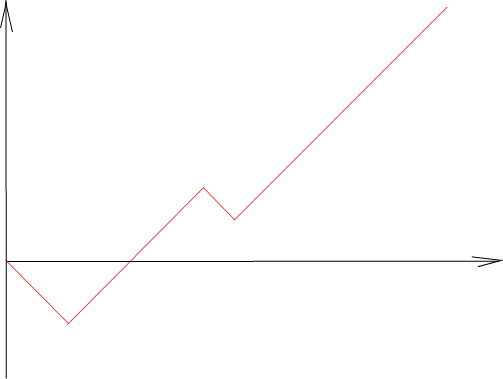
\includegraphics[width=.4\textwidth]{./pictures/4_4.png}
  \caption{График случайноо блуждания}
  \label{fig:44}
\end{figure}

$$S_n =
  \sum \limits_{i = 1}^n \varepsilon_i.$$
Найдём математическое ожидание этого процесса
$$MS_n =
  M \sum \limits_{i = 1}^n \varepsilon_i =$$
Пользуемся независимостью
$$= \sum \limits_{i = 1}^n M \varepsilon_i =
  0,$$
так как
$$M \varepsilon_i =
  1 \cdot \frac{1}{2} - 1 \cdot \frac{1}{2} =
  0.$$
Теперь найдём ковариационную функцию, то есть нужно найти
$$cov \left( S_m, S_t \right) =
  cov \left( \sum \limits_{i = 1}^n \varepsilon_i, \sum \limits_{j = 1}^t \varepsilon_j \right) =$$
Вынесем суммы за ковариацию
$$= \sum \limits_{i = 1}^n \sum \limits_{j = 1}^t cov \left( \varepsilon_i, \varepsilon_j \right) =
\sum \limits_{i, j = 1}^{n, t} M \left( \varepsilon_i \varepsilon_j \right) =$$
Такое математическое ожадине равно
$$M \left( \varepsilon_i \varepsilon_j \right) =
  \begin{cases}
    1, \qquad i = j, \\
    0, \qquad i \neq j.
  \end{cases}$$
Тут пар одинаковых чисел $ \min \left( n, t \right) $, так что
$$= \min \left( n, t \right).$$

По центральной предельной теореме
$$ \frac{S_n}{ \sqrt{n}} \to N \left( 0, 1 \right), \,
  n \to \infty,$$
потому что $S_n$ --- сумма независимых одинаково распределённых случайных величин.

\subsubsection*{4.5}

\textit{Задание.}
Рассмотрим двумерные случайные векторы
$$X^k = \left( \frac{1}{ \sqrt{k}} \cdot S_{ \frac{k}{1}}, \frac{1}{ \sqrt{k}} \cdot S_k \right), \,
  k = 2, 4, 6, \dotsc,$$
где $ \left\{ S_n \right\}_{n \geq 1}$ является простым случайным блужданием.
\begin{enumerate}[label=\alph*)]
  \item Убедитесь, что характеристическая функция вектора $X^k$ имеет вид
  $$ \varphi_{X^k} \left( \theta_1, \theta_2 \right) =
    \left[ \cos \left( \frac{ \theta_1 + \theta_2}{ \sqrt{k}} \right) \right]^{ \frac{k}{2}}
    \left[ \cos \left( \frac{ \theta_2}{ \sqrt{k}} \right) \right]^{ \frac{k}{2}}.$$
  \item Восплользовавшись тем, что
  $$ \varepsilon^{-2} ln \left( \cos \left( \varepsilon \right) \right) \to
    - \frac{1}{2}$$
  при $ \varepsilon \to 0$,
  найдите предел $ \varphi_{X^k} \left( \theta_1, \theta_2 \right) $ при $k \to \infty $
  и укажите распределение случайного вектора $X$,
  к которому слабо сходятся $X^k$ при $k \to \infty$.
\end{enumerate}

\textit{Решение.}
\begin{enumerate}[label=\alph*)]
  \item Сначала нужно найти характеристическую функцию такого вектора
  $ \varphi_{X^{k}} \left( \theta_1, \theta_2 \right) =
    Me^{i \left( \theta_1 X_1^k + \theta_2 X_2^k \right) } $.
  Подставим компоненты
  $$Me^{i \left( \theta_1 X_1^k + \theta_2 X_2^k \right) } =
    Me^{i\left(\theta_1\cdot\frac{1}{\sqrt{k}}\cdot S_{\frac{k}{2}}+\theta_2\cdot\frac{1}{\sqrt{k}}\cdot S_k\right)}.$$
  Можно вынести дробь с корнем от $k$, вместо $S$ будем писать сумму
  $Me^{i\left(\theta_1\cdot\frac{1}{\sqrt{k}}\cdot S_{\frac{k}{2}}+\theta_2\cdot\frac{1}{\sqrt{k}}\cdot S_k\right)} =
    Me^{i\cdot\frac{1}{\sqrt{k}}\left(\theta_1\sum\limits_{i=1}^{\frac{k}{2}}\varepsilon_i +\theta+2\sum\limits_{i = 1}^k\varepsilon_i\right)}$.
  Вторую сумму можно разложить на две
  $$Me^{i\cdot\frac{1}{\sqrt{k}}\left(\theta_1\sum\limits_{i=1}^{\frac{k}{2}}\varepsilon_i +\theta+2\sum\limits_{i = 1}^k\varepsilon_i\right)} =
    Me^{i\cdot\frac{1}{\sqrt{k}}\left(\sum\limits_{i=1}^{\frac{k}{2}}\varepsilon_i\left(\theta_1+\theta_2\right)+\theta_2\sum\limits_{i=\frac{k}{2}+1}^k \varepsilon_i\right)} =$$
  Суммы и слагаемые в суммах независимы
  $$= Me^{i\cdot\frac{1}{\sqrt{k}}\sum\limits_{i=1}^{\frac{k}{2}}\varepsilon_i\left(\theta_1+\theta_2\right)}
    Me^{i \cdot \frac{1}{ \sqrt{k}} \sum \limits_{i = \frac{k}{2} + 1}^k \varepsilon_i \theta_2} =$$
  Все слагаемые в суммах независимы.
  Первое и второе математическое ожидания - произведение $k / 2$ характеристических функций
  \begin{gather*}
    = \prod \limits_{i = 1}^{ \frac{k}{2}}
      \varphi_{ \varepsilon_i} \left( \frac{ \theta_1 + \theta_2}{ \sqrt{k}} \right) \cdot
    \prod \limits_{i = \frac{k}{2} + 1}^k
      \varphi_{ \varepsilon_i} \left( \frac{ \theta_2}{ \sqrt{k}} \right) =
    \end{gather*}
  Осталось понять,
  что такое $ \varphi_{ \varepsilon_i} \left( \lambda \right) = Me^{i \lambda \varepsilon_i}$.
  Случайная величина $ \varepsilon_i$ принимает значения $-1$ и $1$ с вероятностями $0.5$, потому
  $$Me^{i \lambda \varepsilon_i} =
    \frac{1}{2} \cdot e^{i \lambda } + \frac{1}{2} \cdot e^{-i \lambda } =
    \cos \lambda.$$
  Тогда
  $$= \cos^{ \frac{k}{2}} \left( \frac{ \theta_1 + \theta_2}{ \sqrt{k}} \right)
    \cos^{ \frac{k}{2}} \left( \frac{ \theta_2}{ \sqrt{k}} \right).$$
  \item Найдём предел этой характеристической функции, когда $k \to \infty $.

  Оказывается, что
  $$ \varepsilon^{-2} ln \left( \cos \varepsilon \right) \overset{ \varepsilon \to 0}{ \to }
    \frac{1}{2}.$$
  Когда $ \varepsilon \to 0, \, \cos \varepsilon \to 1$ и
  $ln \left( \cos \varepsilon \right) \to 0$ --- это неопределённость 0 на 0.
  Она раскрывается с помощью правила Лопиталя
  $$ \frac{ln \left( \cos \varepsilon \right) }{ \varepsilon^2} \approx
    -\frac{1}{2 \cos \varepsilon } \cdot \frac{ \sin \varepsilon }{ \varepsilon } \to
    \frac{1}{2},$$
  где
  $$ \frac{ \sin \varepsilon }{ \varepsilon }$$
  --- замечательный предел.
  $$ \left( \cos \frac{x}{ \sqrt{k}} \right)^k =
    e^{k \, ln \cos \frac{x}{ \sqrt{k}}} =$$
  Заметим, что
  $$ \frac{x}{ \sqrt{k}} =
    \varepsilon \to
    0,$$
  тогда
  $$= e^{ \frac{k \varepsilon^2 ln \left( \cos \varepsilon \right) }{ \varepsilon^2}} =$$
  Здесь
  $$ \frac{ln \left( \cos \varepsilon \right) }{ \varepsilon^2} \to
    -\frac{1}{2}.$$
  Тогда
  $$= \lim \limits_{ \varepsilon \to 0}
    e^{x^2 \varepsilon^{-2} ln \left( \cos \varepsilon \right) } =
  e^{-\frac{x^2}{2}}.$$
  Теперь нужно эту сходимость использовать
  \begin{gather*}
    \lim \limits_{k \to \infty }
      \cos^{ \frac{k}{2}} \left( \frac{ \theta_1 + \theta_2}{ \sqrt{k}} \right)
      \cos^{ \frac{k}{2}} \left( \frac{ \theta_2}{ \sqrt{k}} \right) =
    e^{-\frac{ \left( \theta_1 + \theta_2 \right)^2}{4}} e^{-\frac{ \theta_2^2}{4}} =
    e^{ \frac{-\theta_1^2 - 2 \theta_1 \theta_2 - \theta_2^2 - \theta_2^2}{4}} = \\
    = e^{-\frac{ \theta_1^2 + 2 \theta_1 \theta_2 + 2 \theta_2^2}{4}}.
  \end{gather*}

  Вывод:
  $$ \varphi_{X^k} \left( \theta_1, \theta_2 \right) \to
    e^{-\frac{1}{4} \left( \theta_1^2 + 2 \theta_1 \theta_2 + 2 \theta_2^2 \right) } =$$
  Это характеристическая функция нормального распределения.
  Оно характеризуется средним и ковариационной матрицей.
  Среднее тут 0, потому что $i$ нет в пределе
  $$= exp \left\{ -\frac{1}{2} \left( A \vec{ \theta }, \vec{ \theta } \right) \right\},$$
  где
  $$ \begin{bmatrix}
      \frac{1}{2} & \frac{1}{2} \\
      \frac{1}{2} & 1
    \end{bmatrix}$$
  --- ковариационная матрица.

  Двумерный случай блуждания сходится к двумерному гауссовскому вектору (рис. \ref{fig:45})
  $$X^k =
    \left( \frac{1}{ \sqrt{k}} \cdot S_{ \frac{k}{2}}, \frac{1}{ \sqrt{k}} \cdot S_k \right) =
    \frac{1}{ \sqrt{k}} \left( S_{k \cdot \frac{1}{2}}, S_{k \cdot 1} \right).$$

  \begin{figure}[h!]
    \centering
    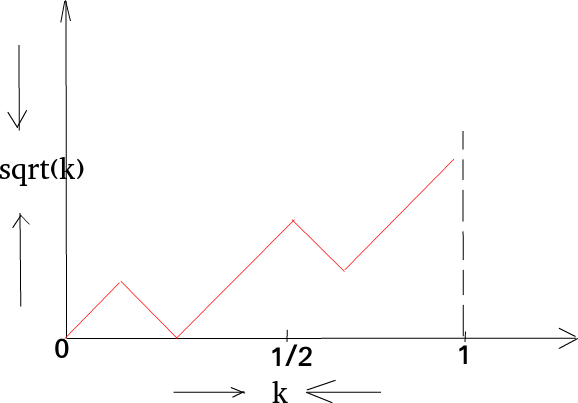
\includegraphics[width=.4\textwidth]{./pictures/4_5.png}
    \caption{Двумерный случай блуждания}
    \label{fig:45}
  \end{figure}

  Если брать не 2 значения, а $n$, то это сходится к
  $$N \left(
      \begin{bmatrix}
        0 \\
        \dotsc \\
        0
      \end{bmatrix},
      \begin{bmatrix}
        t_1 & t_1 & \dotsc & t_1 \\
        \dotsc \\
        t_1 & t_2 & \dotsc & t_n
      \end{bmatrix}
    \right) $$
  --- винеровский процесс.
\end{enumerate}

\subsubsection*{4.6}

\textit{Задание.}
Пусть $ \xi = \left\{ \xi \left( t \right), \, t \geq 0 \right\} $ ---
гауссовский процесс с функцией математического ожидания $m \left( t \right) = t$
и ковариационной функцией
$$K \left( t, s \right) =
  \begin{cases}
    1 - \left| t - s \right|, \qquad \left| t - s \right| < \frac{1}{2}, \\
    \frac{3}{5} - \frac{ \left| t - s \right| }{5}, \qquad \frac{1}{2} \leq \left|t-s\right| < 3, \\
    0, \qquad \left| t - s \right| \geq 3;
  \end{cases}
  t, s \in \mathbb{R}.$$
\begin{enumerate}[label=\alph*)]
  \item Запишите плотность распределения вектора
  $ \left( \xi \left( 1 \right), \xi \left( 3 \right), \xi \left( 4 \right) \right) $.
  \item Найдите условное математическое ожидание
  $M \left(
    \xi \left( 1 \right) \; \middle| \; \left( \xi \left( 3 \right), \xi \left( 4 \right) \right)
  \right) $.
\end{enumerate}

\textit{Решение.}
\begin{enumerate}[label=\alph*)]
  \item Нужно найти плотность трёхмерного вектора
  $ \left( \xi \left( 1 \right), \xi \left( 3 \right), \xi \left( 4 \right) \right) $.
  Процесс гауссовский, значит, такой вектор тоже гауссовский.
  Он характеризуется математическим ожиданием и ковариационной матрицей
  $cov \left( \xi \left( 1 \right), \xi \left( 1 \right) \right) = K \left( 1, 1 \right) $.
  Будем считать по первой строчке.
  Разность равна нулю $K \left( 1, 1 \right) = 1$.
  Аналогично считаем
  $$cov \left( \xi \left( 1 \right), \xi \left( 3 \right) \right) =
    K \left( 1, 3 \right) =
    \frac{1}{5}.$$
  Тогда
  $$ \left( \xi \left( 1 \right), \xi \left( 3 \right), \xi \left( 4 \right) \right)  \sim
    N \left(
      \begin{bmatrix}
        1 \\
        3 \\
        4
      \end{bmatrix},
      \begin{bmatrix}
        1 & \frac{1}{5} & 0 \\
        \frac{1}{5} & 1 & \frac{2}{5} \\
        0 & \frac{2}{5} & 1
      \end{bmatrix}
    \right),$$
  где $cov \left( \xi \left( 1 \right), \xi \left( 4 \right) \right) = K \left( 1, 4 \right) = 0$ и
  $$cov \left( \xi \left( 3 \right), \xi \left( 4 \right) \right) =
    K \left( 3, 4 \right) =
    \frac{2}{5}.$$

  Плотность по определению равна
  $$p \left( \vec{x} \right) =
    \frac{1}{ \sqrt{2 \pi }^3 \sqrt{det \, A}} \cdot
    exp \left\{ -\frac{1}{2}
      \left[ \left( \vec{x} - \vec{m} \right), A^{-1} \left( \vec{x} - \vec{m} \right)
      \right] \right\} =$$
  Чтобы плотность написать, нужно найти определитель матрицы и обратную
  $$det \, A =
    1 - \frac{4}{25} - \frac{1}{5} \cdot \frac{1}{5} =
    \frac{21}{25} - \frac{1}{25} =
    \frac{20}{25} =
    \frac{4}{5}.$$
  Обратная матрица имеет вид
  $$A^{-1} =
    \frac{5}{4}
    \begin{bmatrix}
      \frac{21}{25} & -\frac{1}{5} & \frac{2}{25} \\
      -\frac{1}{5} & 1 & \frac{2}{5} \\
      \frac{2}{25} & \frac{2}{5} & \frac{24}{25}
    \end{bmatrix}.$$
  Тогда плотность равна
  \begin{gather*}
    = \frac{1}{ \sqrt{8 \pi^3 \cdot \frac{4}{5}}} \times \\
    \times exp\{ -\frac{5}{8}
      ( \frac{21}{25} \left( x_1 - 1 \right)^2 + \left( x_2 - 3 \right)^2 +
      \frac{24}{25} \left( x_3 - 4 \right)^2 - \\
      - \frac{2}{5} \left( x_1 - 1 \right) \left( x_2 - 3 \right) +
      \frac{2}{25} \left( x_1 - 1 \right) \left( x_3 - 4 \right) +
      \frac{4}{5} \left( x_2 - 3 \right) \left( x_3 - 4 \right) )\}.
  \end{gather*}

  Здесь
  $$ \vec{x} - \vec{m} =
    \begin{bmatrix}
      x_1 - 1 \\
      x_2 - 3 \\
      x_3 - 4
    \end{bmatrix}.$$
  \item По определению
  $$M \left(
      \xi \left( 1 \right) \; \middle| \; \left( \xi \left( 3 \right), \xi \left( 4 \right) \right)
    \right) =
    \frac{\int\limits_{-\infty}^{+\infty}x_1 p\left(x_1,\xi\left(3\right),\xi\left(4\right)\right)dx_1}{\int\limits_{-\infty}^{+\infty}p\left(x_1,\xi\left(3\right),\xi\left(4\right)\right)dx_1}.$$
  По теореме о нормальной корреляции
  \begin{gather*}
    M \left(
      \xi \left( 1 \right) \; \middle| \; \left( \xi \left( 3 \right), \xi \left( 4 \right) \right)
    \right) = \\
    = M \xi \left( 1 \right) +
    cov_{ \xi \left( 1 \right), \left( \xi \left( 3 \right), \xi \left( 4 \right) \right) } \cdot
    cov_{ \left( \xi \left( 3 \right), \xi \left( 4 \right) \right),
      \left( \xi \left( 3 \right), \xi \left( 4 \right) \right)^{-1}} \cdot
    \begin{bmatrix}
      \xi \left( 3 \right) - M \xi \left( 3 \right) \\
      \xi \left( 4 \right) - M \xi \left( 4 \right)
    \end{bmatrix} =
  \end{gather*}
  Здесь
  $$cov_{ \xi \left( 1 \right), \left( \xi \left( 3 \right), \xi \left( 4 \right) \right) } =
    \begin{bmatrix}
      \frac{1}{5} & 0
    \end{bmatrix}, \,
    cov_{ \left( \xi \left( 3 \right), \xi \left( 4 \right) \right),
      \left( \xi \left( 3 \right), \xi \left( 4 \right) \right)^{-1}} =
    \begin{bmatrix}
      1 & \frac{2}{5} \\
      \frac{2}{5} & 1
    \end{bmatrix}.$$
  Тогда
  \begin{gather*}
    = 1 +
    \begin{bmatrix}
      \frac{1}{5} & 0
    \end{bmatrix}
    \begin{bmatrix}
      1 & \frac{2}{5} \\
      \frac{2}{5} & 1
    \end{bmatrix}^{-1}
    \begin{bmatrix}
      \xi \left( 3 \right) - 3 \\
      \xi \left( 4 \right) - 4
    \end{bmatrix} = \\
    = 1 +
    \begin{bmatrix}
      \frac{1}{5} & 0
    \end{bmatrix} \cdot \frac{25}{21}
    \begin{bmatrix}
      1 & -\frac{2}{5} \\
      \frac{2}{5} & 1
    \end{bmatrix}
    \begin{bmatrix}
      \xi \left( 3 \right) - 3 \\
      \xi \left( 4 \right) - 4
    \end{bmatrix} = \\
    = 1 +
    \begin{bmatrix}
      \frac{5}{21} & 0
    \end{bmatrix}
    \begin{bmatrix}
      \xi \left( 3 \right) - 3 - \frac{2}{5} \cdot \xi \left( 4 \right) + \frac{8}{5} \\
      -\frac{2}{5} \cdot \xi \left( 3 \right) + \frac{6}{5} + \xi \left( 4 \right) - 4
    \end{bmatrix} =
    \frac{5}{21} \cdot \xi \left( 3 \right) - \frac{2}{21} \cdot \xi \left( 4 \right) -
    \frac{2}{3}.
  \end{gather*}
\end{enumerate}

\addcontentsline{toc}{section}{Домашнее задание}
\section*{Домашнее задание}

\subsubsection*{4.10}

\textit{Задание.}
Выясните, существует ли случайный процесс с ковариационной функцией
\begin{enumerate}[label=\alph*)]
  \item $K \left( t, s \right) = \min \left( t, s \right) - ts, \, t, s \in \left[ 0, 1 \right] $;
  \item $K \left( t, s \right) = e^{- \left| t - s \right| }, \, t, s \in \mathbb{R}$.
\end{enumerate}

\textit{Решение.}
\begin{enumerate}[label=\alph*)]
  \item $K \left( t, s \right) = \min \left( t, s \right) - ts, \, t, s \in \left[ 0, 1 \right] $.

  Такой процесс есть.
  Это броуновский мост;
  \item $K \left( t, s \right) = e^{- \left| t - s \right| }, \, t, s \in \mathbb{R}$.

  Симметричность очевидна.
  Вопрос: буде ли такая функция неотрицательно определена?

  Функция зависит только от разности.
  Сейчас $K \left( t, s \right) = \varphi \left( t - s \right) $,
  где $ \varphi \left( t \right) = e^{-\left| t \right| }, \, t \in \mathbb{R}$.

  Так что
  $$ \sum \limits_{k, j = 1}^n c_k c_j K \left( t_k, t_j \right) =
    \sum \limits_{k, j = 1}^n c_k c_j \varphi \left( t_k - t_j \right) \geq
    0$$
  --- это условие неотрицательной определённости для характеристической функции.
  Будет ли эта функция $ \varphi $ характеристической?
  То есть вопрос в задаче равносилен следующему:
  будет ли $ \varphi \left( t \right) = e^{-\left| t \right| }, \, t \in \mathbb{R}$
  характеристической функцией?
  Это характеристическая функция для распределения Коши.
\end{enumerate}

\subsubsection*{4.11}

\textit{Задание.}
Докажите, что функция $K \left( t, s \right) = e^{ts}$
является ковариационной функцией некоторого случайного процесса.

\textit{Решение.}
Симметричность есть.
Вопрос: будет ли такая функция неотрицательно определёной
$$ \sum \limits_{k, j = 1}^n c_k c_j K \left( t_k, t_j \right) =
  \sum \limits_{k, j = 1}^n c_k c_j e^{t_k t_j} =
  \sum \limits_{k, j = 1}^n \left( \sum \limits_{i = 0}^{ \infty } \frac{t_k^i t_j^i}{i!} \right) =
  \sum \limits_{i = 0}^{ \infty } \frac{1}{i!} \sum \limits_{k, j = 1}^n c_k c_j t_k^i t_j^i =$$
Разобьём двойную сумму на две
$$= \sum \limits_{i = 0}^{ \infty } \frac{1}{i!} \sum \limits_{k = 1}^n c_k t_k^i
  \sum \limits_{j = 1}^n c_j t_j^i =
  \sum \limits_{i = 0}^{ \infty } \frac{1}{i!} \left( \sum \limits_{k = 1}^n c_k t_k \right)^i \geq
  0,$$
следовательно, $K \left( t, s \right) = e^{ts}$ --- ковариационная функция.

\subsubsection*{4.12}

\textit{Задание.}
Пусть $ \varphi_1, \dotsc, \varphi_n$ --- произвольные действительные функции,
$c_1, \dotsc, c_n$ --- неотрицательные числа.
Докажите, что функция
$$K \left( t, s \right) =
  \sum \limits_{i = 1}^n c_i \varphi_i \left( t \right) \varphi_i \left( s \right) $$
является ковариационной функцией некоторого случайного процесса.

\textit{Решение.}
Симметричность очевидна.
Вопрос: будет ли такая функция неотрицательно определённой?
$$ \sum \limits_{k, j = 1}^n \lambda_k \lambda_j \sum \limits_{i = 1}^n K \left( t_k, t_j \right) =
  \sum \limits_{k, j = 1}^n \lambda_k \lambda_j
  \sum \limits_{i = 1}^n c_i \varphi_i \left( t_k \right) \varphi_i \left( t_j \right) =$$
Поменяем суммы местами и двойную сумму распишем как две отдельные
$$= \sum \limits_{i = 1}^n c_i \sum \limits_{k = 1}^n \lambda_k \varphi_i \left( t_k \right)
  \sum \limits_{j = 1}^n \lambda_j \varphi_i \left( t_j \right) =
  \sum \limits_{i = 1}^n c_i
    \sum \limits_{k = 1}^n \left( \lambda_k \varphi_i \left( t_k \right) \right)^2 \geq
  0.$$

Значит, функция ковариационная.


\subsubsection*{4.13}

\textit{Задание.}
Пусть случайные величины $X$ и $Y$ имеют совместное гауссовское распределение.
Докажите, что процесс $ \xi \left( t \right) = tX + y, \, t \geq 0$ гауссовский.
Найдите его математическое ожидание и ковариационную функцию.

\textit{Решение.}
$ \xi \left( t \right) $ --- гауссовский, если
$$ \forall \vec{ \alpha } \in \mathbb{R}^n \qquad
  \left( \vec{ \alpha }, \vec{ \xi } \right) = \sum \limits_{i = 1}^n \alpha_i \xi_i$$
--- гауссовская случайная величина, то есть
$$ \sum \limits_{i = 1}^n \xi \left( t_i \right) \alpha_i =
  \sum \limits_{i = 1}^n \left( t_i X + Y \right) \alpha_i =
  X \sum \limits_{i = 1}^n t_i \alpha_i + Y \sum \limits_{i = 1}^n \alpha_i$$
--- сумма гауссовских случайных величин, гауссовская, $ \forall t_1, \dotsc, t_n \geq 0$.

Математическое ожидание $M \xi \left( t \right) = M \left( tX + Y \right) = tMX + My$.

Ковариационная функция
\begin{gather*}
  K \left( t, s \right) = \\
  = M \left[ \xi \left( t \right) \xi \left( s \right) \right] -
  M \xi \left( t \right) M \xi \left( s \right)
  M \left[ \left( tX + Y \right) \left( sX + Y \right) \right] - \\
  - M \left( tX + Y \right) M \left( sX + Y \right) = \\
  = tsMX^2 + tM \left( XY \right) + sM \left( XY \right) + MY^2 -
  \left( tMX + MY \right) \left( sMX + MY \right) = \\
  = tsMX^2 + \left( t + s \right) M \left( XY \right) + MY^2 - ts \left( MX \right)^2 -
  tMX \cdot MY - sMY \cdot MX - \\
  - \left( MY \right)^2 =
  tsDX + DY + \left( t + s \right) D \left( XY \right).
\end{gather*}

\subsubsection*{4.14}

\textit{Задание.}
Пусть $ \left\{ S_n, \, n = 0, 1, 2, \dotsc \right\} $ является случайным блужданием,
которое определяется следующим образом: $S_0 = 0; \, S_{n + 1} = S_n + \xi_{n + 1}$,
где $ \left\{ \xi_n \right\}_{n \geq 1}$ ---
последовательность независимых одинаково распределённых случайных величин таких,
что $M \left[ \xi \right] = 0, \, M \left[ \xi^2 \right] = 1$.
Докажите, что для произвольного фиксированного
$$t \in \left[ 0, 1 \right] \qquad
  \frac{S_{ \left[ nt \right] }}{ \sqrt{n}} \overset{d}{ \to } N \left( 0, t \right), \,
  n \to \infty.$$

\textit{Решение.}
\begin{gather*}
  S_1 = S_0 + \xi_1 = 0 + \xi_1 = \xi_1, \\
  S_2 = S_1 + \xi_2 = \xi_1 + \xi_2, \\
  S_3 = S_2 + \xi_3 = \xi_1 + \xi_2 + \xi_3, \\
  \dotsc, \\
  S_n = \sum \limits_{i = 1}^n \xi_i.
\end{gather*}

Математическое ожидание
$$MS_n =
  M \sum \limits_{i = 1}^n \xi_i =
  \sum \limits_{i = 1}^n M \xi_i =
  nM \xi_i =
  0.$$

Дисперсия
$$DS_n =
  D \sum \limits_{i = 1}^n \xi_i =
  \sum \limits_{i = 1}^n D \xi_i =
  nD \xi_i =
  n.$$

Значит, по центральной предельной теореме
$$ \frac{S_{ \left[ nt \right] }}{ \sqrt{n}} \overset{d}{ \to } N \left( 0, t \right), \,
  n \to \infty.$$
